\section{Rendimiento \emph{Clúster}}

\subsection{Variación número de hilos en el \emph{clúster}}

\begin{itemize}
    \item \textbf{Simulación:} G4pntest
    \item \textbf{Número de neutrones:} \num{10e6}
    \item \textbf{Energía:} 0.025 eV
    \item \textbf{Variación de Número de hilos con:} open MPI
    \item \textbf{Número de computadores:} 6
    \item \textbf{Número de hilos disponibles:} 48
    \item \textbf{Comando:} \$mpirun -np 3 -hostfile ./PNtest THEmacro.mac    
\end{itemize}

\begin{figure}[htb]
	\centering
	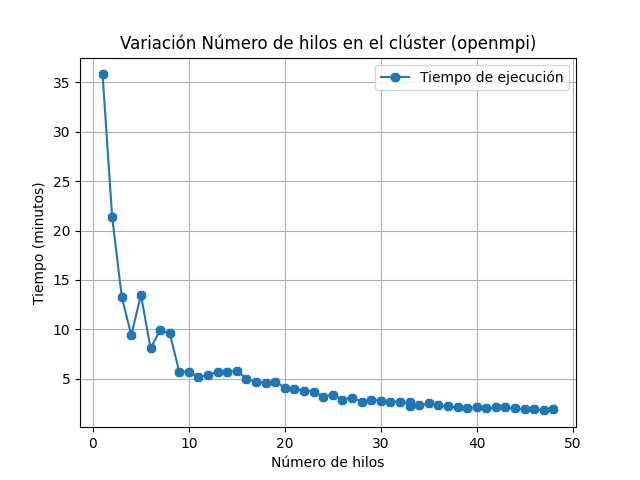
\includegraphics[width=0.9\textwidth]{images/hilos_openmpi.png}
	%caption{\scriptsize{Medición tiempo de ejecución variando el número de hilos en la aplicación}}
	\label{fig:AntennaDesign}
\end{figure}




% \begin{figure}[htb]
% 	\centering
% 	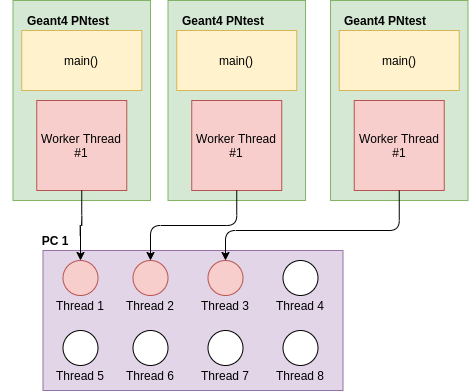
\includegraphics[width=0.5\textwidth]{images/Diagram_hilos_openmpi.png}
% 	%\caption{\scriptsize{Medición tiempo de ejecución variando el número de hilos en la aplicación}}
% 	\label{fig:AntennaDesign}
% \end{figure}





\newpage

\subsection{Comparación Clúster vs 1 PC, variando el número de neutrones}

\begin{itemize}
    \item \textbf{Simulación:} G4pntest
    \item \textbf{Energía:} 0.025 eV
    \item \textbf{Número de neutrones:} \num{200e6}
    \item \textbf{Número de hilos utilizados en PC:} 8 
    \item \textbf{Número de hilos utilizados en el Clúster:} 48
    
\end{itemize}


\begin{table}[H]
\centering
\begin{tabular}{|l|c|c|c|}
\hline
                                      & \textbf{\begin{tabular}[c]{@{}c@{}}PC\\ (Geant4MT)\end{tabular}} & \textbf{\begin{tabular}[c]{@{}c@{}}Clúster\\ (open MPI)\end{tabular}} & \textbf{\begin{tabular}[c]{@{}c@{}}Aceleración\\ Clúster\end{tabular}} \\ \hline
\multicolumn{1}{|c|}{\textbf{Tiempo}} & 1 hora 36 minutos                                                & 42 minutos                                                            & 2.3 veces más rápida                                                   \\ \hline
\end{tabular}
\end{table}

\newpage

\subsection{Comparación Resultados de una simulación usando MT y MPI}
Simulación con $1x10^6$ neutrones disparados directamente al suelo en un cono con apertura angular de 85 grados:

La energía de los neutrones sigue la distribución de la fuente de 252Cf. El detector es un cilindro con dimensiones $5x100$ cm2 alto x diámetro

\begin{itemize}
    \item \textbf{Simulación:} G4pntest
    \item \textbf{Energía:} 0.025 eV
    \item \textbf{Número de neutrones:} \num{1e6}
    \item \textbf{Número de hilos utilizados con MT:} 60 
    \item \textbf{Número de hilos utilizados en el Clúster:} 40
    
\end{itemize}


\begin{figure}[htb]
	\centering
	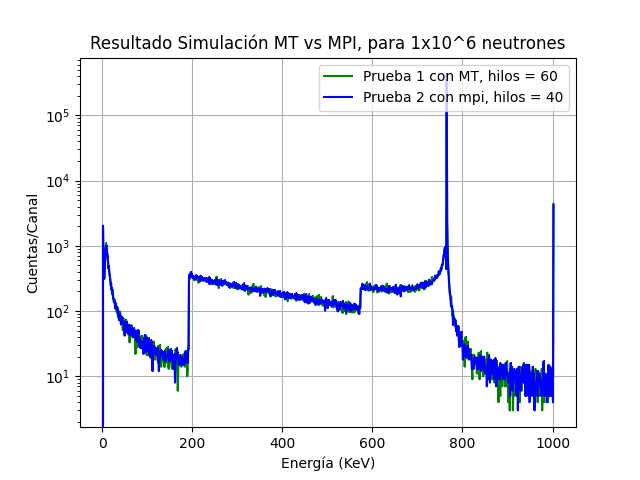
\includegraphics[width=0.9\textwidth]{images/test_MT_vs_Cluster.png}
	%caption{\scriptsize{Medición tiempo de ejecución variando el número de hilos en la aplicación}}
	\label{fig:AntennaDesign}
\end{figure}

